% Author: Alfredo Sánchez Alberca (asalber@ceu.es)
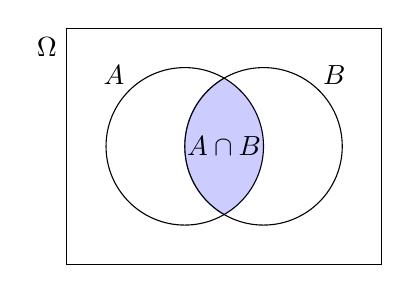
\begin{tikzpicture}
\def\firstcircle{(-0.5,0) circle (1cm)}
\def\secondcircle{(0.5,0) circle (1cm)}

\begin{scope}
\clip \firstcircle;
\fill[fill=blue!20, draw=blue!60] \secondcircle;
\end{scope}

\draw (-2,1.5) node[anchor=north east] {$\Omega$} rectangle (2,-1.5);
\draw \firstcircle node[xshift=-0.9cm, yshift=0.9cm] {$A$};
\draw \secondcircle node[xshift=0.9cm, yshift=0.9cm] {$B$};

\node at (0,0) {$A\cap B$};
\end{tikzpicture}